\documentclass[11pt,a4paper]{article}

\usepackage[T1]{fontenc}
\usepackage[utf8]{inputenc}
\usepackage{lmodern}
\usepackage{microtype}
\usepackage{amsmath,amssymb,amsthm,mathtools,bm}
\usepackage{booktabs,array,tabularx,longtable}
\usepackage{graphicx,float,caption}
\usepackage{xcolor}
\usepackage[margin=23mm]{geometry}
\usepackage{enumitem}
\usepackage{fancyhdr}
\usepackage{hyperref}

\definecolor{finblue}{HTML}{1F5A99}
\definecolor{finorange}{HTML}{C45A00}
\definecolor{fingreen}{HTML}{19733A}
\definecolor{finred}{HTML}{A61B1B}
\definecolor{finpurple}{HTML}{6B3FA0}
\definecolor{finsoft}{HTML}{F2F5F8}
\definecolor{fingray}{HTML}{4E5964}

\hypersetup{
  colorlinks=true,
  linkcolor=finblue,
  citecolor=fingreen,
  urlcolor=finblue,
  pdftitle={FIN Programs P497-P506: Localization and Identifiability},
  pdfauthor={Krzysztof Żuchowski},
  pdfsubject={Localized strict-DNLS states, certified spectral stability, phase topology, passivity, operational and trajectory identifiability},
  pdfkeywords={FIN, nadsoliton, DNLS, anti-continuum, localization, interval stability, relational clock, Stieltjes inverse, winding, identifiability}
}

\pagestyle{fancy}
\fancyhf{}
\fancyhead[L]{\small FIN Programs P497--P506}
\fancyhead[R]{\small Release 10.50}
\fancyfoot[C]{\thepage}
\setlength{\headheight}{14pt}

\newtheorem{theorem}{Theorem}[section]
\newtheorem{proposition}[theorem]{Proposition}
\newtheorem{corollary}[theorem]{Corollary}
\theoremstyle{definition}
\newtheorem{definition}[theorem]{Definition}
\theoremstyle{remark}
\newtheorem{remark}[theorem]{Remark}

\newcommand{\C}{\mathbb C}
\newcommand{\R}{\mathbb R}
\newcommand{\Z}{\mathbb Z}
\newcommand{\one}{\bm 1}
\newcommand{\status}[2]{\textcolor{#1}{\textbf{[#2]}}}
\newcommand{\proven}{\status{fingreen}{PROVEN}}
\newcommand{\strong}{\status{finblue}{STRONG EVIDENCE}}
\newcommand{\moderate}{\status{finorange}{MODERATE EVIDENCE}}
\newcommand{\speculative}{\status{finpurple}{SPECULATIVE}}
\newcommand{\refuted}{\status{finred}{REFUTED}}
\newcommand{\conditional}{\status{fingray}{CONDITIONAL}}
\newcommand{\claimbox}[1]{\begin{center}\fcolorbox{finblue}{finsoft}{\parbox{0.91\textwidth}{#1}}\end{center}}

\setlist[itemize]{leftmargin=*,topsep=3pt,itemsep=2pt}
\setlist[enumerate]{leftmargin=*,topsep=3pt,itemsep=2pt}
\setlength{\emergencystretch}{2em}

\begin{document}
\hypersetup{pageanchor=false}

\begin{titlepage}
\centering
\vspace*{15mm}
{\Huge\bfseries FIN Programs P497--P506\par}
\vspace{5mm}
{\Large Localization, Certified Stability, Phase Topology,\par}
{\Large and Identifiability\par}
\vspace{4mm}
{\large A bounded analytical and small-compute continuation of Release 10.49\par}
\vspace{15mm}
{\Large Krzysztof Żuchowski\par}
\vspace{2mm}
{\normalsize Independent Researcher --- Fractal Information Theory Project\par}
{\normalsize ORCID: 0009-0002-0909-3613\par}
\vspace{10mm}
{\large FIN Release 10.50 --- Version 1.0.0\par}
{\large 10 August 2026\par}
\vfill
\begin{minipage}{0.90\textwidth}
\small
\textbf{Scope.} This report executes all ten low-compute recommendations P497--P506 from Release 10.49. The stopped P485/P487 Gröbner campaign and global exact complex-cone problems remain excluded.

\medskip
\textbf{Evidence boundary.} Analytic theorems, outward interval evaluation, finite numerical continuation, FFT quadrature and synthetic records are admitted. A supplied nonlinear law is never promoted to a consequence of FIN. No laboratory or external-audit evidence is claimed.

\medskip
\textbf{Runtime.} The complete deterministic batch ran locally in approximately 21 seconds. Twelve regression and certificate tests passed.

\medskip
\textbf{Repository.} \url{https://github.com/hyconiek/Fractal-Nadsoliton-Theory}

\textbf{License.} CC BY 4.0.
\end{minipage}
\vfill
\end{titlepage}
\hypersetup{pageanchor=true}

\begin{abstract}
Ten bounded FIN studies are executed. The principal result is conditional but mathematically substantive. For the supplied focusing discrete nonlinear Schrödinger law
\[
 i\dot\psi=\kappa A\psi-|\psi|^2\psi,
\]
the strict $\Z_{12}$ generator admits a one-site anti-continuum state whose stationary Jacobian is exactly $\operatorname{diag}(-2,1,\ldots,1)$. The implicit-function theorem therefore produces a unique local real branch. Numerical continuation reaches the full strict coupling $\kappa=1$ without a break and with residual $2.22\times10^{-16}$, inverse participation ratio $0.654578$, and central-site power fraction $0.804496$. This is a localized nonlinear state, unlike the delocalized cycles of P488. It is not yet a FIN-derived physical nadsoliton because the focusing cubic law and frequency are supplied.

The P488 spectral stability calculation is reduced analytically to $2\times2$ Fourier blocks and evaluated by outward interval arithmetic. Every nonzero real exponent is strictly negative in the declared decimal strict model; mode three retains an additional exact neutral block. A two-frequency clock theorem proves periodicity precisely for rational frequency ratio and injectivity for irrational ratio. For the strict first two frequencies, rationals with denominator at most $10^6$ are excluded by an outward interval certificate, but global irrationality remains open.

The Stieltjes inverse problem receives a local rational-left-inverse certificate. It proves local injectivity only inside a log-parameter box of radius $10^{-9}$ and for response noise below $1.17\times10^{-16}$, quantitatively confirming severe practical fragility. The even/odd context family is extended through $C_{192}$ and $C_{384}$ and compared with a polyphase integral fingerprint; the $C_{384}$ discrepancy is $0.003244$ and decreases monotonically after $C_{96}$.

The Legacy*--strict linear parameter homotopy has two distinct boundaries. Its signed Laplacian becomes positive semidefinite near $t=0.7008185569$, whereas all six radial weights become nonnegative only at the exact $d=6$ phase crossing $t=0.9257900390$. A nonvanishing $S^1$ phase field with branch-cut margin is then constructed; bounded updates and geodesic refinement preserve integer winding exactly. Finally, one context from the P495 synthetic catalogue suffices to distinguish its four models, while a trajectory no-go proves that no finite set of kernel observations can identify a unique continuous parameter evolution law.

The batch therefore supplies a credible conditional localization mechanism, completes several certification tasks, and sharpens the missing-law boundary. It does not derive the cubic nonlinearity, absolute units, a selector, the legacy-to-strict parameter source, laboratory physics, particles, or a Theory of Everything.
\end{abstract}

\noindent\textbf{Status vocabulary.}
\proven{} means an analytic statement or exact finite proof in its declared assumptions;
\strong{} means robust numerical or synthetic evidence;
\conditional{} marks dependence on a supplied dynamical or operational law;
\moderate{} marks bounded evidence that is not a global theorem;
\refuted{} marks a scoped no-go or counterexample.

\tableofcontents
\newpage

\section{Executive results}

\claimbox{\textbf{Principal advance.} P497 crosses the localization boundary left open by P488. A focusing strict-DNLS branch exists rigorously near zero coupling and remains strongly localized in numerical continuation to full strict coupling. The advance concerns the mathematical capability of the strict generator after a cubic law is supplied; it does not derive that law from FIN.}

\begin{longtable}{@{}p{0.07\textwidth}p{0.24\textwidth}p{0.39\textwidth}p{0.22\textwidth}@{}}
\caption{Programs, typed objects, and terminal verdicts.}\\
\toprule
ID & New object & Main result & Status\\
\midrule
\endfirsthead
\toprule
ID & New object & Main result & Status\\
\midrule
\endhead
P497 & O201 strict-DNLS localization branch & Local IFT theorem and full-coupling numerical localization, IPR $0.654578$. & \conditional{} / \strong\\
P498 & O202 Fourier-block stability enclosure & All nonzero P488 real exponents are interval-enclosed below zero; one extra neutral block for $m=3$. & \proven\\
P499 & O203 two-frequency torus clock & Rational/irrational dichotomy proven; no rational with denominator $\le10^6$ for the strict interval. & \proven{} / \moderate\\
P500 & O204 Stieltjes inverse box & Local inverse certified, but only at extremely small noise and parameter radius. & \conditional{}\\
P501 & O205 polyphase integral fingerprint & $C_{192},C_{384}$ approach a declared asymptotic integral fingerprint. & \strong\\
P502 & O206 passivity/PSD boundary ledger & Exact radial boundary $0.9257900390$ differs from PSD boundary $0.7008185569$. & \proven{} / \strong\\
P503 & O207 nonvanishing phase-refinement sector & Bounded updates and midpoint refinement preserve winding. & \proven\\
P504 & O208 one-context coherence tester & One catalogue context separates four synthetic models with $99.925\%$ simulated accuracy. & \strong\\
P505 & O209 neutral theorem interface & Six theorem nodes pass schema and dependency-DAG validation. & \proven{} in interface scope\\
P506 & O210 trajectory observation quotient & Static parameters are locally observable; finite records never identify a unique continuous path. & \proven{} / \strong\\
\bottomrule
\end{longtable}

\section{Shared strict finite core and kernel discipline}

On $V=\Z/12\Z$, let
\[
 W_{xy}=\frac{\cos(0.18575d(x,y)+0.16250)}{1+d(x,y)^{1.8}},\qquad
 A=\operatorname{diag}(W\one)-W.
\]
The row sum of $W$ is $1.6603072787660986\ldots$, all six strict radial weights are positive, and $A\succeq0$. This report uses $A$ only as the later strict working generator. It does not identify it silently with
\[
 K_{\rm legacy}(d)=4\ln2\,\frac{\cos(\pi d/4+\pi/6)}{1+0.01d}
\]
or transfer any legacy electromagnetic, hierarchy, Planck-scale, or matter role.

\section{P497 --- localized nonlinear strict states}

\subsection{The supplied DNLS object}

Consider the focusing finite DNLS equation
\begin{equation}
 i\dot\psi=\kappa A\psi-g|\psi|^2\psi,qquad g=1,quad 0\le\kappa\le1.
 \label{eq:dnls}
\end{equation}
With $\psi(t)=e^{-i\mu t}u$, $\mu=-1$ and real $u$, the stationary equation is
\begin{equation}
 F(u,\kappa)=\kappa Au-u^{\circ3}-\mu u=0.
 \label{eq:stationary}
\end{equation}

\begin{theorem}[Anti-continuum persistence]
At $\kappa=0$, the state $u_0=(1,0,\ldots,0)$ solves \eqref{eq:stationary}. There is a unique real stationary branch through $u_0$ for all sufficiently small $|\kappa|$.
\end{theorem}
\begin{proof}
At $(u_0,0)$,
\[
 D_uF=-3\operatorname{diag}(u_0^2)-\mu I
      =\operatorname{diag}(-2,1,\ldots,1).
\]
It is invertible, so the finite-dimensional implicit-function theorem applies.
\end{proof}

This is the theorem-level part of P497. The extension from a nonzero neighbourhood of $\kappa=0$ to $\kappa=1$ is a numerical continuation result, not a global continuation proof.

\begin{table}[H]
\centering
\caption{Selected points on the continued branch.}
\begin{tabular}{@{}rrrrr@{}}
\toprule
$\kappa$ & power & IPR & peak fraction & $\|F\|_\infty$\\
\midrule
0.00 & 1.000000 & 1.000000 & 1.000000 & 0\\
0.25 & 1.420032 & 0.954169 & 0.976737 & $2.22\times10^{-16}$\\
0.50 & 1.863852 & 0.863450 & 0.928550 & $2.22\times10^{-16}$\\
0.75 & 2.346621 & 0.759523 & 0.869404 & $2.22\times10^{-16}$\\
1.00 & 2.881677 & 0.654578 & 0.804496 & $2.22\times10^{-16}$\\
\bottomrule
\end{tabular}
\end{table}

\begin{figure}[H]
\centering
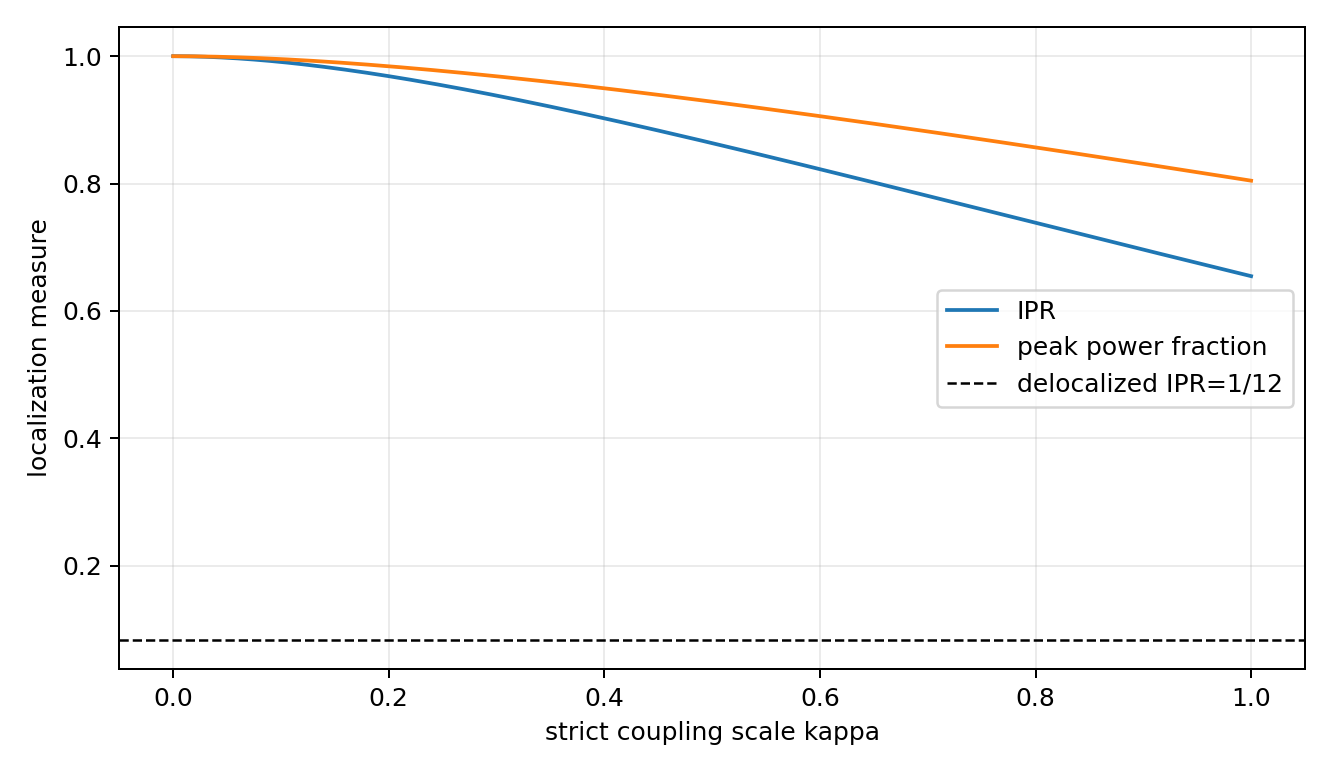
\includegraphics[width=0.78\textwidth]{FIN_Programs_497_506_Figures/p497_localization_branch.png}
\caption{Localization decreases continuously as strict coupling is turned on, but remains far above the delocalized value $1/12$ at $\kappa=1$.}
\end{figure}

\begin{figure}[H]
\centering
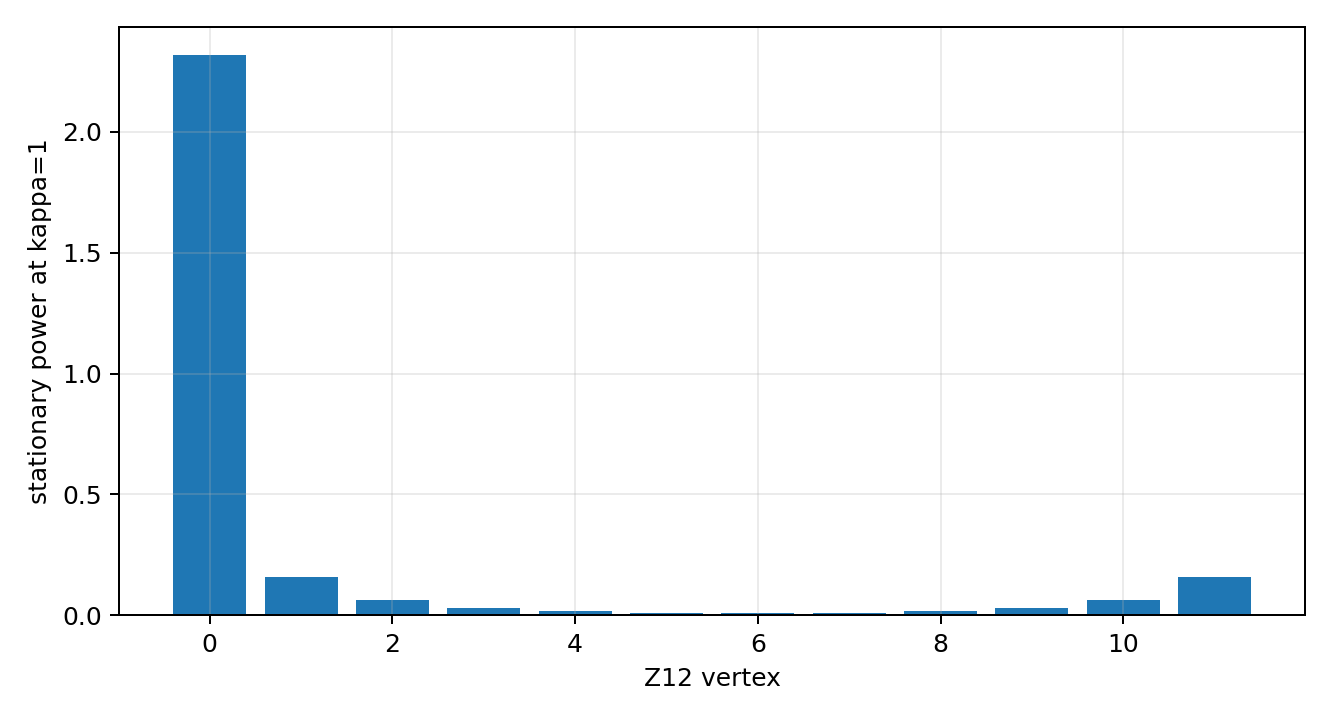
\includegraphics[width=0.78\textwidth]{FIN_Programs_497_506_Figures/p497_endpoint_profile.png}
\caption{Power profile at full strict coupling. The state is pinned at the selected vertex; translation produces eleven equivalent copies.}
\end{figure}

The Hamiltonian linearization has no resolved real exponent above $10^{-6}$ along the sampled branch, but near-zero Hamiltonian eigenvalues require a separate orbital-stability certificate. Therefore asymptotic stability is not claimed. Nor is mobility: a pinned discrete breather is not yet a travelling soliton.

\paragraph{P497 verdict.} \conditional{} local persistence is proven for the supplied DNLS; \strong{} full-coupling localization is numerically established. The source and sign of the cubic law, the choice $\mu=-1$, continuum persistence, orbital stability and physical interpretation remain open.

\section{P498 --- interval certification of P488 stability}

Let $\lambda_j$ be the strict Fourier eigenvalues and let $m$ label a persistent P488 background. Fourier perturbations with offsets $q$ and $-q$ reduce the real $24\times24$ linearization to $2\times2$ blocks. If
\[
 d_{m,q}=\frac{\lambda_{m+q}+\lambda_{m-q}-2\lambda_m}{2},
\]
then the two block exponents have real parts
\begin{equation}
 \Re\rho_{m,q}^{\pm}=-r\pm\Re\sqrt{r^2-d_{m,q}^2},\qquad r=0.2.
 \label{eq:block}
\end{equation}
All strict weights and eigenvalues were evaluated with 70-decimal outward interval arithmetic.

\begin{table}[H]
\centering
\caption{Largest certified upper bound among nonzero real parts for each excited background.}
\begin{tabular}{@{}rrr@{}}
\toprule
mode $m$ & largest nonzero upper bound & exact neutral offsets\\
\midrule
1 & $-0.0029812392$ & $q=0$\\
2 & $-0.0065292023$ & $q=0$\\
3 & $-0.0138368211$ & $q=0,6$\\
4 & $-0.0124870968$ & $q=0$\\
5 & $-0.0019318268$ & $q=0$\\
6 & $-0.0048048352$ & $q=0$\\
\bottomrule
\end{tabular}
\end{table}

The $q=0$ block is global phase neutrality. For $m=3,q=6$, inversion symmetry gives $\lambda_{m+q}=\lambda_{m-q}=\lambda_m$, so the second neutrality is exact rather than a rounding accident. P498 upgrades P488's nonzero transverse signs, but it correctly refuses asymptotic stability for mode three because of that additional neutral direction.

\section{P499 --- two-frequency clock atlas}

\begin{theorem}[Torus clock dichotomy]
For nonzero $\omega_1,\omega_2$, the map
\[
 t\longmapsto(e^{-i\omega_1t},e^{-i\omega_2t})\in\mathbb T^2
\]
has a nonzero period if and only if $\omega_2/\omega_1\in\mathbb Q$. If the ratio is irrational, the map is injective on $\R$.
\end{theorem}
\begin{proof}
A repeated value at times $t$ and $t+T$ requires both $\omega_1T$ and $\omega_2T$ to be integer multiples of $2\pi$. A nonzero common $T$ exists exactly when the frequency ratio is rational.
\end{proof}

For the strict modes,
\[
 \omega_1=0.7541211542070798,\qquad
 \omega_2=1.5770495144276093,
\]
and outward interval evaluation gives
\[
 2.0912415805200384\le\omega_2/\omega_1
 \le2.0912415805200393.
\]
For every $1\le q\le10^6$, the interval $q[\omega_2/\omega_1]$ excludes all integers. The smallest paid separation is $1.2852\times10^{-7}$ at $q=740693$. Thus no rational with denominator at most $10^6$ is possible. This is not a proof of irrationality.

\begin{figure}[H]
\centering
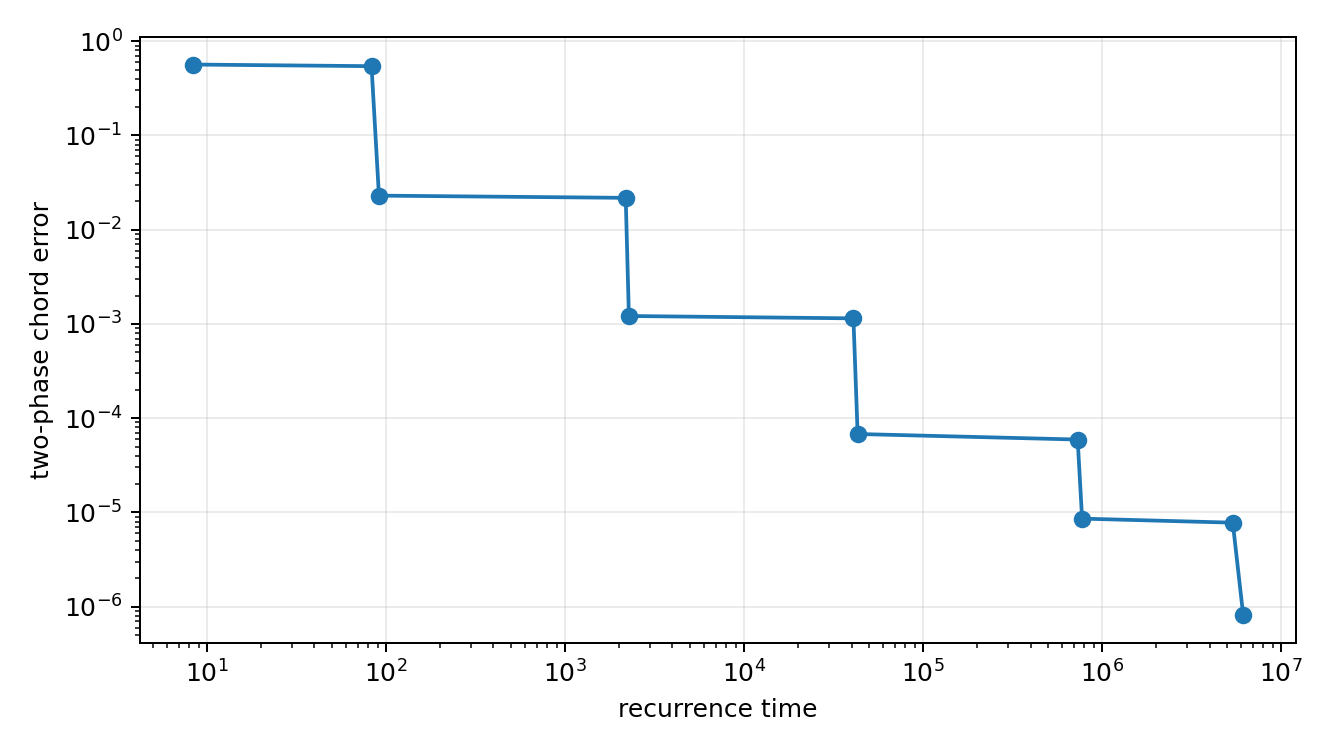
\includegraphics[width=0.76\textwidth]{FIN_Programs_497_506_Figures/p499_clock_recurrence.png}
\caption{Continued-fraction recurrence quality. Small phase error is purchased with a rapidly increasing dimensionless waiting time.}
\end{figure}

The best audited recurrence has dimensionless time $6.1713\times10^6$ and two-phase chord error $8.09\times10^{-7}$. Like P489, this clock is dimensionless and invariant under common generator/time rescaling.

\section{P500 --- Stieltjes identifiability bounds}

The three-pole response is
\[
 \sigma(z;\theta)=\sum_{j=1}^3\frac{e^{b_j}}{z+e^{a_j}},
 \qquad \theta=(a_1,a_2,a_3,b_1,b_2,b_3).
\]
Let $F$ be the 48-component relative response map at the P490 sampling points. A rational approximation $R$ to the left inverse of $J_0=DF(\theta_*)$ was constructed with denominator at most $10^{12}$. Interval evaluation on the box $\|\theta-\theta_*\|_\infty\le10^{-9}$ gives
\[
 \|RDF(\theta)-I\|_F\le q=0.245562333<1.
\]

\begin{proposition}[Local inverse bound]
Throughout this box,
\[
 \|F(\theta)-F(\theta_*)\|_2
 \ge c\|\theta-\theta_*\|_2,qquad
 c=\frac{1-q}{\|R\|_F}=1.17160\times10^{-7}.
\]
\end{proposition}
\begin{proof}
Integrate $DF$ on the segment from $\theta_*$ to $\theta$, multiply by $R$, and use the triangle inequality with $\|RDF-I\|_2\le\|RDF-I\|_F\le q$ and $\|Rv\|_2\le\|R\|_F\|v\|_2$.
\end{proof}

The self-consistency condition requires response-noise norm below
\[
 c\times10^{-9}=1.17160\times10^{-16}.
\]
The condition number is $3.4729\times10^7$. Thus local uniqueness exists in a narrow mathematical sense, while ordinary finite-precision pole recovery is fragile. The certificate is conditional on the declared rounded P490 poles, residues, contexts and response definition.

\section{P501 --- context-family limit}

For the summable attenuation envelope $h_d=(1+d^{1.8})^{-1}$, split the infinite lattice into even and odd sites. Let $C(\theta)$ be the odd--odd Laplacian symbol plus $\delta=0.1$, and $B(\theta)$ the even--odd symbol. The limiting trace response is
\begin{equation}
 \sigma(z)=\frac1{2\pi}\int_0^{2\pi}
 \frac{|B(\theta)|^2}{z+C(\theta)}\,d\theta.
 \label{eq:polyphase}
\end{equation}
The formula follows by diagonalizing the two polyphase convolution blocks with the Fourier transform. It supplies a natural continuum-context object; it does not supply exact finite self-similarity.

\begin{table}[H]
\centering
\caption{Maximum normalized-fingerprint discrepancy from the FFT approximation of \eqref{eq:polyphase}.}
\begin{tabular}{@{}rr@{}}
\toprule
cycle & maximum discrepancy\\
\midrule
$C_{12}$ & 0.0372626\\
$C_{24}$ & 0.0312736\\
$C_{48}$ & 0.0183403\\
$C_{96}$ & 0.0102133\\
$C_{192}$ & 0.00574028\\
$C_{384}$ & 0.00324399\\
\bottomrule
\end{tabular}
\end{table}

\begin{figure}[H]
\centering
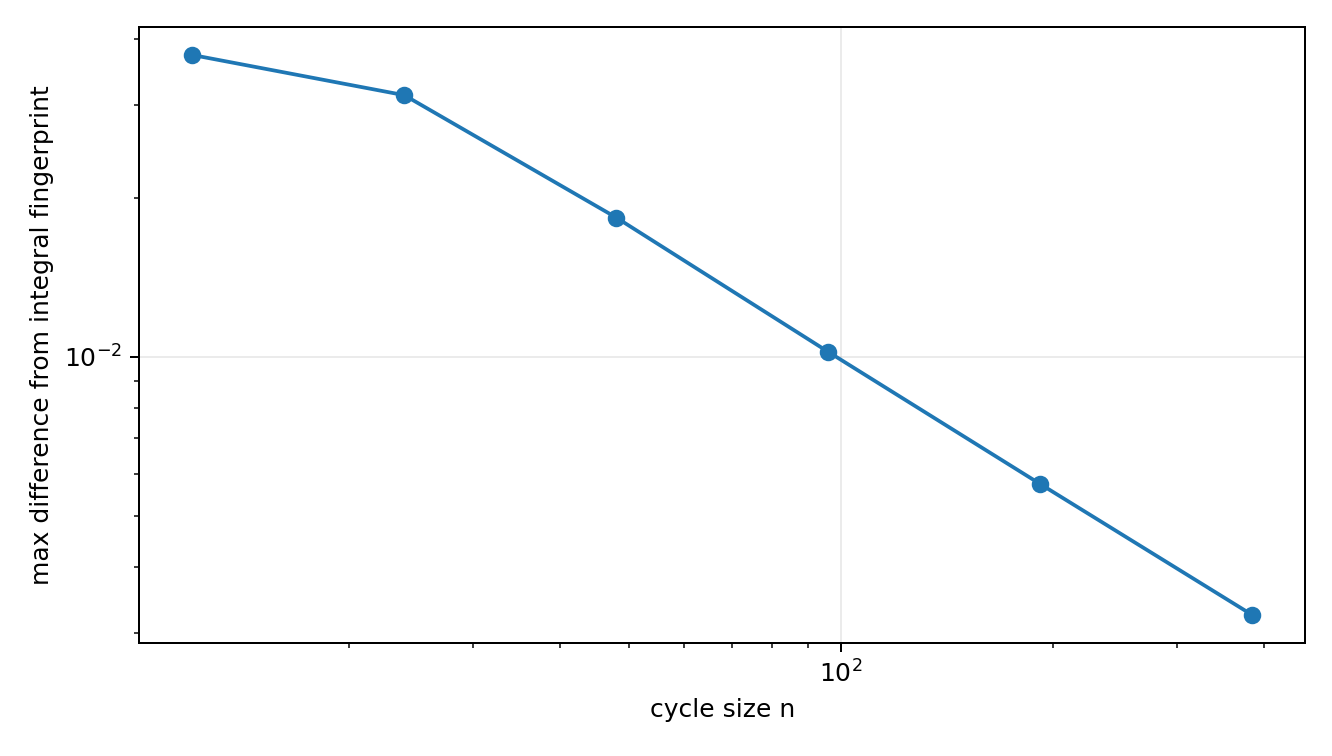
\includegraphics[width=0.76\textwidth]{FIN_Programs_497_506_Figures/p501_context_limit.png}
\caption{Approach to the declared polyphase integral fingerprint. The omitted infinite weight $\ell^1$ tail in the $C_{131072}$ proxy is bounded by $3.51\times10^{-4}$; this is not itself a bound on the nonlinear normalized fingerprint error.}
\end{figure}

The discrepancy decreases monotonically from $C_{96}$ onward. This is strong convergence evidence for this particular envelope and context, not a universal fractal theorem.

\section{P502 --- exact radial passivity and signed PSD}

Along the linear parameter homotopy from Legacy* to strict, the amplitude and denominator remain positive. Hence the sign of the $d$th radial weight is the sign of
\[
 \cos\big((1-t)(\pi d/4+\pi/6)+t(0.18575d+0.16250)\big).
\]
The last crossing into the final nonnegative sector is at $d=6$:
\begin{equation}
 t_{\rm radial}=
 \frac{5\pi/3-\pi/2}{5\pi/3-(6\cdot0.18575+0.16250)}
 =0.9257900390444757\ldots .
\end{equation}
It is isolated in
\[
 [0.9257900390439756,\;0.9257900390449756],
\]
where the limiting radial weight changes from $-1.02\times10^{-13}$ to $+1.02\times10^{-13}$.

The signed Laplacian can be PSD before every weight is nonnegative. Auditing all eleven nonconstant Fourier eigenvalues gives the last PSD crossing in mode one:
\[
 t_{\rm PSD}\in[0.7008185569041573,\;0.7008185569051574].
\]
The minimum nonzero eigenvalue changes sign across the bracket. Thus
\[
 t_{\rm PSD}<t_{\rm radial}.
\]
This distinction matters: PSD is a collective spectral property; pointwise radial passivity is a stronger sufficient condition. Neither boundary makes the arbitrary linear parameter homotopy a derivation of strict from legacy.

\section{P503 --- a nonvanishing phase refinement sector}

P494 showed that unconstrained scalar states in $\C^{12}$ have no protected winding. P503 adds exactly the missing typed structure.

\begin{definition}
Let $z_x\in S^1$ and
\[
 \Delta_x=\operatorname{Arg}(z_{x+1}\overline z_x)\in(-\pi,\pi).
\]
If every edge stays off the branch cut, define
\[
 \nu(z)=\frac1{2\pi}\sum_x\Delta_x\in\Z.
\]
\end{definition}

\begin{theorem}[Bounded-update and refinement invariance]
Suppose $|\Delta_x|\le\pi-\varepsilon$ and an update has a real lift $\delta_x$ satisfying $|\delta_{x+1}-\delta_x|<\varepsilon$ on every cyclic edge. Then $z'_x=e^{i\delta_x}z_x$ satisfies $\nu(z')=\nu(z)$. Inserting on every edge the principal-geodesic midpoint also preserves $\nu$ and halves every edge increment.
\end{theorem}
\begin{proof}
The bound prevents a principal-argument branch crossing. Therefore
\[
 \Delta'_x=\Delta_x+\delta_{x+1}-\delta_x.
\]
Summation telescopes on the cycle. Midpoint refinement replaces each $\Delta_x$ by two increments $\Delta_x/2$.
\end{proof}

The implementation replayed 1500 bounded random updates on $C_{12},C_{24},C_{48}$ with zero failures. It also found a condition-violating update changing winding from $1$ to $-1$. P503 therefore constructs a mathematically protected phase sector, but the phase field, branch margin and update law are extra axioms. No particle interpretation follows automatically.

\section{P504 --- minimal synthetic coherence tester}

All 36 single contexts of the P495 catalogue were exhausted. Nine individually separate its four declared models. The strongest one-context design is
\[
 t=0.55,\qquad \rho_0=|\widehat1\rangle\langle\widehat1|,
 \qquad \text{Fourier-basis measurement}.
\]
Its minimum pairwise total-variation separation is $0.235223$. With 120 shots, the sum of pairwise Bhattacharyya error bounds is $0.012807$. A deterministic-seed simulation of 1000 trials per model gave
\[
\begin{pmatrix}
1000&0&0&0\\
0&1000&0&0\\
0&0&998&2\\
0&0&1&999
\end{pmatrix},
\qquad \text{accuracy}=0.99925.
\]

\begin{figure}[H]
\centering
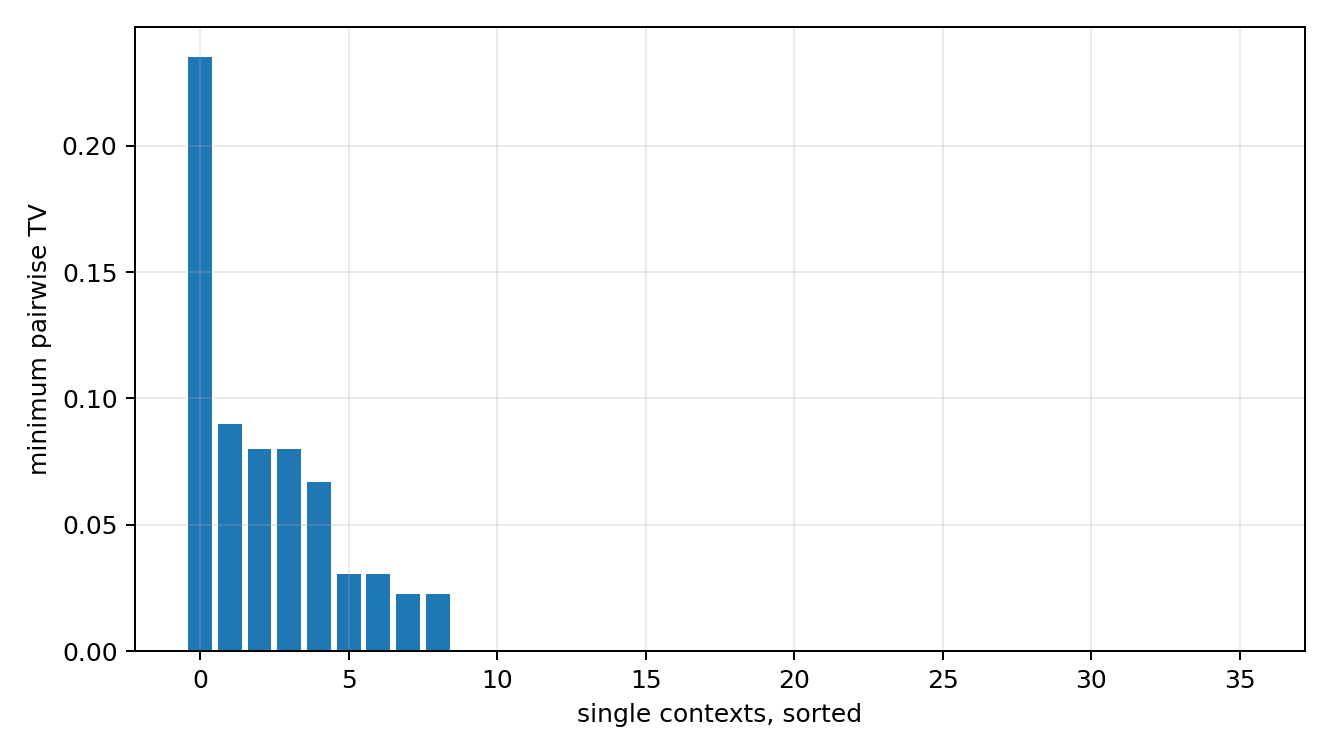
\includegraphics[width=0.76\textwidth]{FIN_Programs_497_506_Figures/p504_single_context_separation.png}
\caption{Minimum pairwise total variation for all single contexts, sorted. Only nine contexts separate all four synthetic model families.}
\end{figure}

Minimality is exact only within this finite catalogue: zero contexts contain no data and one separating context exists. The models, preparation, time, measurement and shot law remain synthetic inputs.

\section{P505 --- theorem dependency interface}

The file \path{FIN_P497_P506_Theorem_Interface.json} records six theorem nodes:
\[
\begin{aligned}
 &\text{T488-CYCLE},\ \text{T489-SCALE},\ \text{T492-COMPLEMENT},\\
 &\text{T493-INDUCTION},\ \text{T497-IFT},\ \text{T503-WINDING}.
\end{aligned}
\]
Every node contains assumptions, claim level, conclusion, dependencies, proof skeleton and explicit nonclaims. Schema validation found no missing field; dependency validation found no missing node and no cycle. The canonical payload has SHA-256
\begin{center}
\path{79259faf581ecd506124ad1a52465a5fe1e1bc7b95bb8b616ea259598441da81}.
\end{center}
The value above is checked against the generated interface during regression testing. This is a proof-assistant-neutral transfer format, not a Lean/Coq/Isabelle machine proof.

\section{P506 --- parameter-path identifiability no-go}

Write
\[
 K(d;p)=a\frac{\cos(\omega d+\phi)}{1+\beta d^\eta},
 \qquad p=(\log a,\log\beta,\eta,\omega,\phi).
\]
The Jacobian of $(K(0),\ldots,K(6))$ has rank five at the Legacy*, midpoint and strict parameter points. Their respective condition numbers are approximately $1225.8$, $49.87$ and $544.84$. Among five-distance strict designs, the best audited subset is
\[
 d\in\{0,1,2,3,6\},\qquad \kappa(J)=632.75.
\]
Thus a static parameter point is locally identifiable after its phase/positivity branch has been fixed.

\begin{theorem}[Finite-record trajectory no-go]
No observation of a parameter or kernel trajectory at finitely many times $t_1,\ldots,t_M$ identifies a unique continuous parameter trajectory in any open admissible parameter set.
\end{theorem}
\begin{proof}
Let $p(t)$ be one admissible trajectory and choose a nonzero parameter direction $v$. For sufficiently small $\epsilon$,
\[
 \widetilde p(t)=p(t)+\epsilon v\prod_{j=1}^M(t-t_j)^2
\]
is distinct from $p$ but agrees with it at every observation time. Consequently all sampled kernel values agree as well.
\end{proof}

Even a continuously observed unlabelled curve is invariant under monotone time reparameterization. A calibrated continuous time record and a full-rank distance design can recover a path pointwise, but a causal evolution law is still an additional object. P506 therefore rules out deriving the P493 parameter transition from endpoints or any finite set of snapshots.

\section{Integrated interpretation}

\subsection{What has improved}

\begin{enumerate}
\item \textbf{Localization is now mathematically possible.} Strict coupling is compatible with a strongly localized stationary DNLS branch.
\item \textbf{The P488 stability signs are certified.} The earlier floating signs reduce to outward-enclosed $2\times2$ blocks.
\item \textbf{The clock question is sharper.} A two-mode clock removes single-period aliasing conditionally on irrationality, and a large finite rational class is excluded.
\item \textbf{The Stieltjes fragility is quantified.} The numerical condition number now has a local inverse theorem and an explicit noise threshold.
\item \textbf{Approximate context convergence has a target.} The polyphase integral replaces vague fixed-point language by an explicit asymptotic response.
\item \textbf{Passivity notions are separated.} Signed PSD and nonnegative radial coupling are demonstrably different boundaries.
\item \textbf{The topology obligation is fulfilled conditionally.} An $S^1$ phase field plus admissible updates supports protected winding.
\item \textbf{Operational complexity fell sharply.} One synthetic coherence context suffices within the declared catalogue.
\item \textbf{The bridge nonidentifiability is now a theorem.} Static observability does not create a unique parameter evolution law.
\end{enumerate}

\subsection{What has not improved}

\begin{itemize}
\item FIN does not derive the focusing cubic sign, coefficient, or stationary frequency used in P497.
\item Numerical continuation to $\kappa=1$ is not an interval-certified global branch or orbital-stability theorem.
\item The localized state is pinned; mobility and collision persistence are untested.
\item No absolute time, length, action, mass or energy unit is generated.
\item The $S^1$ phase sector is an added object, not a strict selector or $QW$-2191 discharge.
\item The Legacy*--strict homotopy is a diagnostic path, not the missing completion/source theorem.
\item Synthetic identifiability is not preparation, apparatus, calibration, raw data or independent custody.
\item No legacy physical role is transferred to strict.
\end{itemize}

\claimbox{\textbf{Updated scientific interpretation.} The strict kernel has now passed a nontrivial capability test: after a standard focusing Hamiltonian nonlinearity is supplied, it supports a strongly localized finite breather. The decisive missing theorem is therefore no longer ``can this generator localize at all?'' but ``does FIN internally select the nonlinear law, its sign and its scale, and can the resulting localized branch be certified and connected to an observable instrument?''}

\section{Recommended next bounded studies P507--P516}

\begin{longtable}{@{}p{0.09\textwidth}p{0.29\textwidth}p{0.45\textwidth}p{0.09\textwidth}@{}}
\caption{Next local analytical and small-compute programmes.}\\
\toprule
Program & Objective & Acceptance criterion & Priority\\
\midrule
\endfirsthead
\toprule
Program & Objective & Acceptance criterion & Priority\\
\midrule
\endhead
P507 & Source audit for the focusing nonlinearity & Derive the cubic sign/coefficient from an admitted variational or information functional, or prove that the strict quadratic core leaves it free. & 10/10\\
P508 & Certified global DNLS continuation & Cover $0\le\kappa\le1$ by interval root boxes and overlapping IFT charts; reject any unresolved fold. & 10/10\\
P509 & Orbital stability of O201 & Apply a finite-graph Grillakis--Shatah--Strauss/Vakhitov--Kolokolov audit and isolate the near-zero Hamiltonian blocks. & 9/10\\
P510 & Mobility and Peierls--Nabarro barrier & Continue site- and bond-centred branches, compare constrained energies and test whether a moving localized state can exist. & 9/10\\
P511 & Localized spectral-memory dynamics & Couple O201 to the positive Stieltjes state variables of O194 and determine whether localization survives causal memory. & 8/10\\
P512 & Strict frequency-ratio arithmetic & Prove irrationality of $\lambda_2/\lambda_1$ or give a precise transcendence obstruction showing why current theorems cannot decide it. & 8/10\\
P513 & Certified context convergence rate & Bound the normalized fingerprint error using Wiener-algebra and resolvent estimates rather than an FFT proxy alone. & 8/10\\
P514 & Exact signed-PSD homotopy boundary & Interval-certify every Fourier-mode root and prove global PSD/non-PSD on both sides of $t_{\rm PSD}$. & 7/10\\
P515 & Robust one-context tester & Add preparation, timing and POVM uncertainty; retain separation with a worst-case lower TV bound or reject one-context robustness. & 9/10\\
P516 & Minimal trajectory-law observations & Under explicit ODE/gradient-flow model classes, determine the smallest time/distance design that identifies a law rather than only a path. & 9/10\\
\bottomrule
\end{longtable}

P507 and P508 are the immediate priorities. P507 decides whether the localization mechanism belongs to FIN or merely to an added DNLS model. P508 decides whether the attractive numerical branch is a theorem across the complete strict coupling interval.

\section{Reproducibility}

Primary artifacts:
\begin{itemize}
\item \path{fin_programs_497_506_next_research.py};
\item \path{test_fin_programs_497_506.py};
\item \path{FIN_Programs_497_506_Results.json};
\item \path{FIN_Programs_497_506_Summary.csv};
\item \path{FIN_P497_P506_Theorem_Interface.json};
\item \path{FIN_Programs_497_506_Figures/}.
\end{itemize}

Replay commands:
\begin{verbatim}
MPLCONFIGDIR=/tmp/fin-mpl-1050 \
  python3 fin_programs_497_506_next_research.py
MPLCONFIGDIR=/tmp/fin-mpl-1050 \
  python3 -m unittest -v test_fin_programs_497_506.py
pdflatex -interaction=nonstopmode -halt-on-error \
  FIN_Programs_497_506_Localization_and_Identifiability_Report_EN.tex
\end{verbatim}

The main computation uses matrices no larger than $144\times144$, a 12-variable nonlinear stationary solve, FFT arrays of length $131072$, short interval evaluations and a finite 36-context synthetic search. It is suitable for an ordinary local computer.

\section{Final verdict and nonclaims}

The P497--P506 batch makes real progress. The strict generator is compatible with localization once a focusing cubic Hamiltonian term is supplied. The localized branch has a theorem-level origin at the anti-continuum limit and a robust numerical continuation to full strict coupling. Several prior numerical observations have been upgraded: P488 stability signs are interval-enclosed, the Stieltjes inverse has a local bound, the passivity threshold is isolated, and the missing topological state space is explicitly constructed.

The falsification boundary is equally important. Static kernel values can identify parameters locally but cannot identify their evolution law. The focusing term is not derived. The phase field is added. The clock remains dimensionless. The operational tester remains synthetic. These facts prevent the localized state from being promoted to experimentally established matter, a universal informational soliton, or a completed physical theory.

No result in this release discharges $QW$-2191, selects an orientation, generates SI or Planck units, completes the Legacy*--strict bridge, transfers a legacy physical role, supplies laboratory evidence, derives the Standard Model or gravity, constructs $L_{\rm total}$, or closes a Theory of Everything.

\end{document}
